
%%%%%%%%%%%%%%%%%%%%%%% file typeinst.tex %%%%%%%%%%%%%%%%%%%%%%%%%
%
% This is the LaTeX source for the instructions to authors using
% the LaTeX document class 'llncs.cls' for contributions to
% the Lecture Notes in Computer Sciences series.
% http://www.springer.com/lncs       Springer Heidelberg 2006/05/04
%
% It may be used as a template for your own input - copy it
% to a new file with a new name and use it as the basis
% for your article.
%
% NB: the document class 'llncs' has its own and detailed documentation, see
% ftp://ftp.springer.de/data/pubftp/pub/tex/latex/llncs/latex2e/llncsdoc.pdf
%
%%%%%%%%%%%%%%%%%%%%%%%%%%%%%%%%%%%%%%%%%%%%%%%%%%%%%%%%%%%%%%%%%%%


\documentclass[runningheads,a4paper]{llncs}

\usepackage{amssymb}
\setcounter{tocdepth}{3}
\usepackage{graphicx}\usepackage{wrapfig}

\usepackage{url}
\urldef{\mailsa}\path|{alfred.hofmann, ursula.barth, ingrid.haas, frank.holzwarth,|
\urldef{\mailsb}\path|anna.kramer, leonie.kunz, christine.reiss, nicole.sator,|
\urldef{\mailsc}\path|erika.siebert-cole, peter.strasser, lncs}@springer.com|    
\newcommand{\keywords}[1]{\par\addvspace\baselineskip
\noindent\keywordname\enspace\ignorespaces#1}

\begin{document}

\mainmatter  % start of an individual contribution

% first the title is needed
\title{SIMD Acceleration for Main-Memory Index Structures -- A Survey}

% a short form should be given in case it is too long for the running head
\titlerunning{SIMD Acceleration for Index Structures}

% the name(s) of the author(s) follow(s) next
%
% NB: Chinese authors should write their first names(s) in front of
% their surnames. This ensures that the names appear correctly in
% the running heads and the author index.
%
\author{Marten Wallewein-Eising \and David Broneske \and Gunter Saake%
%\thanks{Please note that the LNCS Editorial assumes that all authors have used
%the western naming convention, with given names preceding surnames. This determines
%the structure of the names in the running heads and the author index.}%
%\and Ursula Barth\and Ingrid Haas\and Frank Holzwarth\and\\
%Anna Kramer\and Leonie Kunz\and Christine Rei\ss\and\\
%Nicole Sator\and Erika Siebert-Cole\and Peter Stra\ss er
}
%
\authorrunning{SIMD Acceleration for Index Structures}
% (feature abused for this document to repeat the title also on left hand pages)

% the affiliations are given next; don't give your e-mail address
% unless you accept that it will be published
\institute{University of Magdeburg,\\
Magdeburg, Germany\\
{firstname.lastname}@ovgu.de\\
}

%
% NB: a more complex sample for affiliations and the mapping to the
% corresponding authors can be found in the file "llncs.dem"
% (search for the string "\mainmatter" where a contribution starts).
% "llncs.dem" accompanies the document class "llncs.cls".
%

\toctitle{SIMD Acceleration for Index Structures}
\tocauthor{Authors' Instructions}
\maketitle


\begin{abstract}
	Index structures designed for disk-based database systems do not fulfill the requirements for modern database systems. To improve the performance of these index structures, different approaches are presented by several authors, including horizontal vectorization with SIMD and efficient cache line usage. 
	
	In this work, we compare the adapted index structures Seg-Tree/Trie, FAST, VAST, and ART and evaluate the usage of SIMD within these. We extract important criteria of these adaptions and weight them according to their impact on the performance. Furthermore, we present openings in the considered index structures for additional adaptions to combine advantages of them.
	
	\keywords SIMD, horizontal vectorization
	%\begin{itemize}
	%	\item summary: 
	%	\subitem Give short an overview of SIMD and modern index structures
	%	\subitem Explain what are the problems of the ``old" index structures made for disk-based database systems
	%	\subitem Explain which approaches were made to adapt index structures to modern systems and what they have in common and what are differences
	%	\item Why is this work important: 
	%	\subitem Give a state of current development of the index structures
	%	\subitem Collect common approaches to adapt other index structures TODO: ReThink
	%	\item K-ary search trees, FAST, VAST and ART compared
	%	\item Contribution: What are important approaches used by different implementations to adapt index structures to modern systems
	%\end{itemize}
\end{abstract}

%\begin{IEEEkeywords}
	
%\end{IEEEkeywords}

\section{Introduction}
% Main Problem: Index structures designed for disk-based database systems
After decades of creating and improving index structures for disk-based database systems, nowadays even large databases fit into the main memory. Since index structures like the $B^+$-tree or the radix tree have an important part in database systems to realise scan or range-based search operations, these index structures experienced many adaptions to fulfill the needs of modern database systems. Instead of overcoming the bottleneck of IO-operations from disk to RAM, the target of modern index structures is to improve the usage of CPU cache and processor architectures.

% Introduce tree structures and specific Problem: Cache and TLB misses and branch mispredictions cost a lot of calculation effort
Several index structures have already shown that the bottleneck from RAM to CPU can be overcome using Single Instruction Multiple Data (SIMD) \cite{suaib2011architecture} operations. These index structures include: the k-ary Search Tree (Seg-tree) \cite{zeuch2014adapting}, Adapted Radix Tree (ART) \cite{leis2013adaptive}, Fast Architecture Sensitive Tree (FAST) \cite{kim2010fast}, and Vector-Advanced and Compressed Structure Tree (VAST) \cite{yamamuro2012vast}. As Yamamuro et al. show, important causes for increased runtime are cache misses and branch mispredictions. To overcome branch mispredictions and to decrease CPU cycles, SIMD  is used in modern index structures for tree traversal \cite{zhou2002implementing}. Zeuch et al. show how to use SIMD to compare mutliple keys in one CPU cycle. To decrease cache misses, the Kim et al. and Leis et al. show how they adapted FAST and ART to the cache line size.  

% Objectives and Contribution
All approaches use SIMD only for key comparison within tree traversal and try to decrease the key size to fit more keys into one SIMD register. Therefore FAST and Seg-tree only provide implementations for search algorithms. With this work we make the following contributions:
\begin{itemize}
	\item We compare different adaptions of index structures to fulfill requirements of modern database systems
	\item We highlight the usage of SIMD and the cache line adaptions in all approaches
	\item We extract important points of these adaptions and their performance impact on the index structures
\end{itemize}
% Paper structure
We organized the rest of the paper as follows. In Section 2, we give the preliminaries for SIMD in general and for the use in index structures. In Section 3, we present the different approaches of adapted index structures and compare them in Section 4. In Section 5, we name related work. In Section 6, we present our conclusion and describe future work. 
\section{SIMD-Style Processing}

\begin{wrapfigure}{r}{0.45\textwidth} \vspace{-20pt}
  \begin{center}
	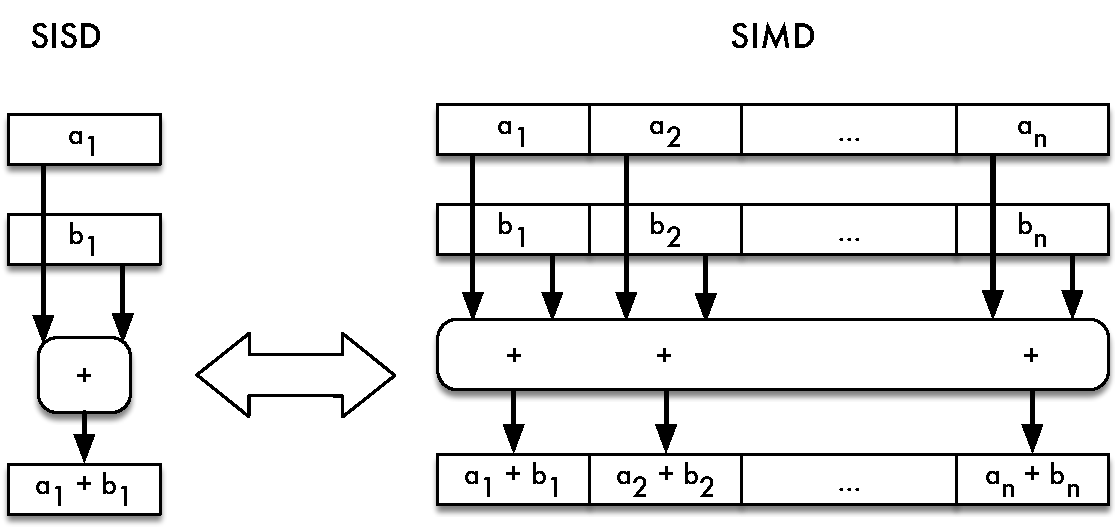
\includegraphics[width=.45\textwidth]{SIMD}
	\caption{Single Instruction Single Data (SISD) vs.\ Single Instruction Multiple Data (SIMD) processing.}
	\label{fig}  \end{center}
  \vspace{-20pt}
\end{wrapfigure} 
% SIMD explanation
A common approach of decreasing CPU cycles for algorithms is to adapt the algorithm to pipelining. While one instruction is executed, the next instruction is already fetched. This approach executes one instruction on one data item, called Single Instruction Single Data (SISD). In contrast to execute one operation on one data item after another, the idea of Single Instruction Multiple Data (SIMD) is to execute a single instruction on multiple data items in parallel. In Figure 1, we show the difference between SIMD and SISD. 

%\begin{table*}[htbp]
%\footnotesize
%	\caption{SIMD instructions from Streaming SIMD Extensions 2 (SSE2)}
%	\begin{center}
%		\begin{tabular}{|c|c|}
%			\hline
%			\textbf{SIMD instruction}&\textbf{Explanation}\\
%			\hline
%			\_\_m128i \_mm\_load\_si128 (\_\_m128i *p) & Loads a 128-bit value. Returns the value loaded into a variable representing a register.\\
%			\_\_m128i \_mm\_cmpgt\_epi32 (\_\_m128i a, \_\_m128i b) & Compares 4 signed 32-bit integers in a and 4 signed 32-bit integers
%			in b for greater-than.\\
%			\_\_m128i \_mm\_set1\_epi32(int i) & Sets the four signed 32-bit integer values to i.\\
%			\hline
%		\end{tabular}
%		\label{tasuaib2011architecture}
%	\end{center}
%\end{table*}
% SIMD explanation
Modern CPUs have additional SIMD registers along with an additional instruction set adapted to process multiple data items in parallel. %In Table 1, we show some SIMD 
For example, using the Streaming SIMD Extensions 2 (SSE2) on the example in Figure~\ref{fig}, we can add 4 values in one clock cycle.
After loading 4 different signed 32-bit integers in register $a$ and 4 signed 32-bit integers in register $b$, we add them using \_mm\_add\_epi32. %The comparison returns a bitmask showing which of the search keys in $a$ is greater than the one in $b$. 

% Pro's/contra's of SIMD
%Consequently, the main advantage of SIMD is to process multiple data items in parallel in contrast to SISD. 
The main restriction of SIMD instructions is that a sequential load of data is required. To load data into a SIMD register, the data has to be stored consecutively in main memory. Additionally, the size of SIMD registers is limited. Therefore processing data types of the common size of 64-bit and more lead to a small performance increase, since only few data items are processed with a single instruction.

% Horizontal vs vertical vector processing
Polychroniou et al. \cite{polychroniou2015rethinking} show two general approaches to use SIMD, horizontal and vertical vector processing. They name the comparison of one search key to multiple other keys horizontal vectorization, whereas processing a different input key per vector lane is named vertical vectorization.

% How horizontal vectorization works
Since FAST, Seg-Tree, ART and VAST only use horizontal vectorization, we focus on this approach.  For example, Zeuch et al. \cite{zeuch2014adapting} use 128-bit SIMD registers and adjusted SIMD operations to load data into a register and to compare the data of one SIMD register with another. For example, a 128-bit SIMD register processes sixteen 8-bit or eight 16-bit data items with one instruction. %In Table 2 TODO: Insert Table! we show a comparison of key size and the number of keys that can be processed parallel with one SIMD instruction.

% SIMD restrictions

\section{Adapted Tree Structures}
In this section, we review the previously proposed index structures Seg-Tree/Trie, FAST, ART, and VAST. We consider the adaptions made compared to the base index structure, the usage of SIMD, and the performance gain presented by the authors of the certain index structures.
\subsection{Seg-Tree and Seg-Trie}\label{SCM}
% Basics k-ary search
Zeuch et al. adapted the $B^+$-Tree by having a k-ary search tree as each inner node, called segment, and perform a k-ary search on each segment.  In Figure 2, we show the adaption of nodes made by Zeuch et al. for Seg-Tree. The k-ary search bases on the binary search but divides the search space into k partitions with k-1 separators. Compared to binary search, the k-ary search reduces the complexity from $O(\log_{2}{n})$ to $O(\log_{k}{n})$. They consider $m$ as the most bits to represent a data type and $\vert SIMD \vert$ as the size of SIMD-register, called SIMD bandwidth. Then, $k = \frac{\vert SIMD \vert }{m}$ defines the number of partitions for the k-ary search. 

\begin{figure}
	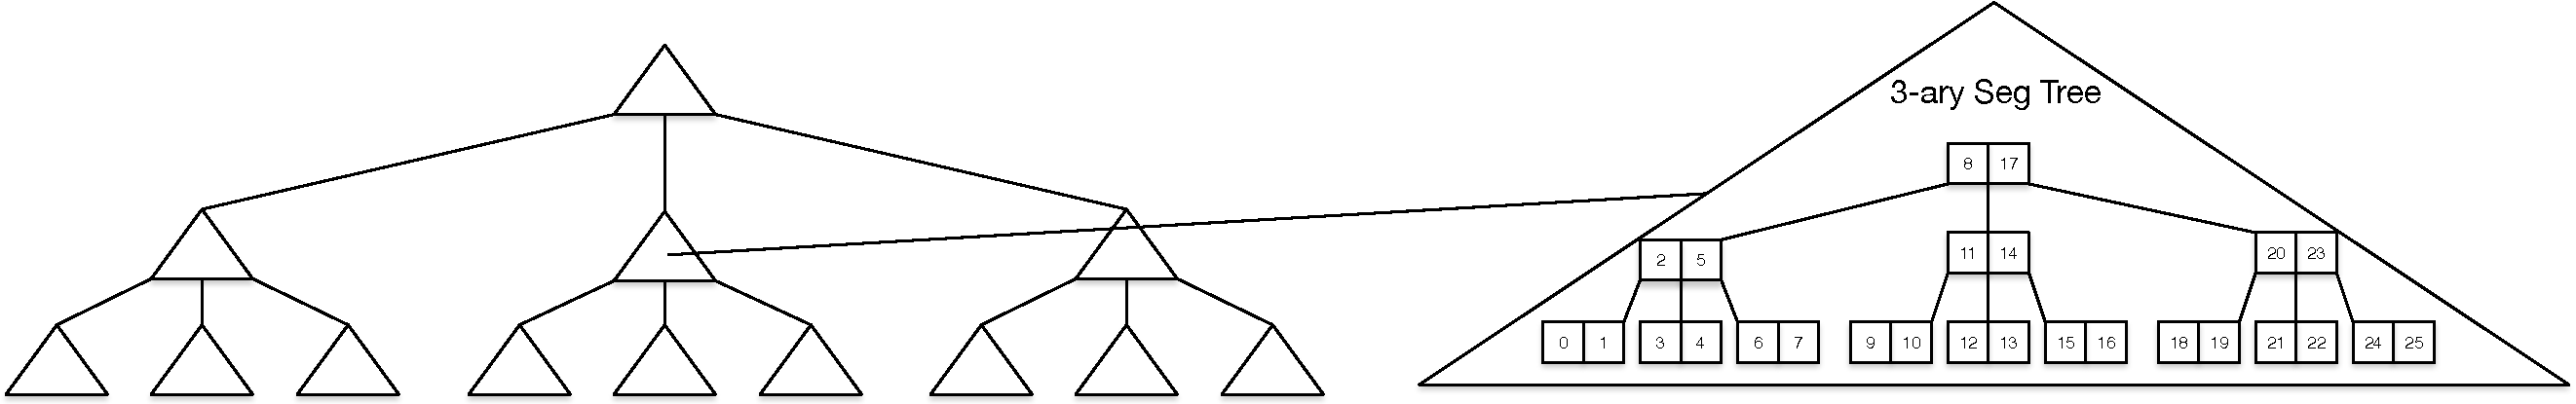
\includegraphics[width=\textwidth]{SegTree}
	\caption{Inner node format of Seg-Tree}
	\label{fig}
\end{figure}

% Performing k-ary search on Seg-tree
As mentioned before, each segment of the Seg-Tree is a k-ary search tree. To perform a k-ary search on a segment, Zeuch et al. linearise the elements of the segment. They show two algorithms for linearisation using breadth-first search and depth-first search. Because of the condition $k = \frac{\vert SIMD \vert }{m}$, each partition of the k-ary search fits into a SIMD register and is compared to the search key. A perfect k-ary search tree contains  $S_{max} = k^h - 1$ keys for an integer $h > 0$. The considered search algorithm only works for sequences with a multiple of $k-1$ keys. In case of  sequences with less than a multiple of $k-1$ keys, they replenish the sequence with elements having the value $k_{max} + 1$ for the maximal key value $k_{max}$ in the sequence. Consequently, the adapted search algorithm works for sequences with less than a multiple of $k-1$ keys.

% Performance increase
The performance of Seg-Tree depends on k-ary search and horizontal vectorization. The smaller a key the more keys are compared parallel. According to the relevance of 32 and 64-bit data types in modern systems, the k-ary search performance increases up to the factor of four for 32-bit types and two for 64-bit types.

% Addional adaption: Seg-trie
%TODO: Each Node is also k-ary search tree
Zeuch et al. also show the k-ary search on an adapted prefix tree \emph{(trie for short)} called Seg-Trie. A trie is a search tree where nodes store a parts of the key, called chunks. For example, a 32 bit key with a chunk size of 8 bit is stored in a trie with 4 levels. Analogue to the Seg-Tree, each node is again designed as a k-ary search tree. Complete keys are stored in leaf nodes or are build by concatenating partial keys from the root node to a leaf node. This approach benefits of the separation of the keys in different levels of the tree. Consequently, they are smaller and more keys can be compared in parallel. The Seg-Trie$_L$ is defined as a balanced trie where each node on each level contains one part of a key with $L$ Bits. The tree has $r = \frac{m}{L}$ levels $(E_0, E_1, .., E_r)$, where m is the number of most bits to represent the data type.

% K-ary search on Seg-Trie
To perform a tree traversal on the Seg-Trie, the search key is split into $r$ segments and each segment $r_i$ is compared to the level $E_i$. If a matching partial key is found in one node of $E_i$, the search continues at the referenced node for the partial key. If no match of the partial key is found, the Seg-Trie does not contain the search key and the search is finished. Consequently, the advantage of Seg-Trie against tree structures is the reduced comparison effort for non-existing key segments. 

% Performance increase of Seg-Trie?

\subsection{FAST}\label{SCM}
% Introduction of FAST
\begin{wrapfigure}{r}{0.45\textwidth} \vspace{-40pt}
  \begin{center}
	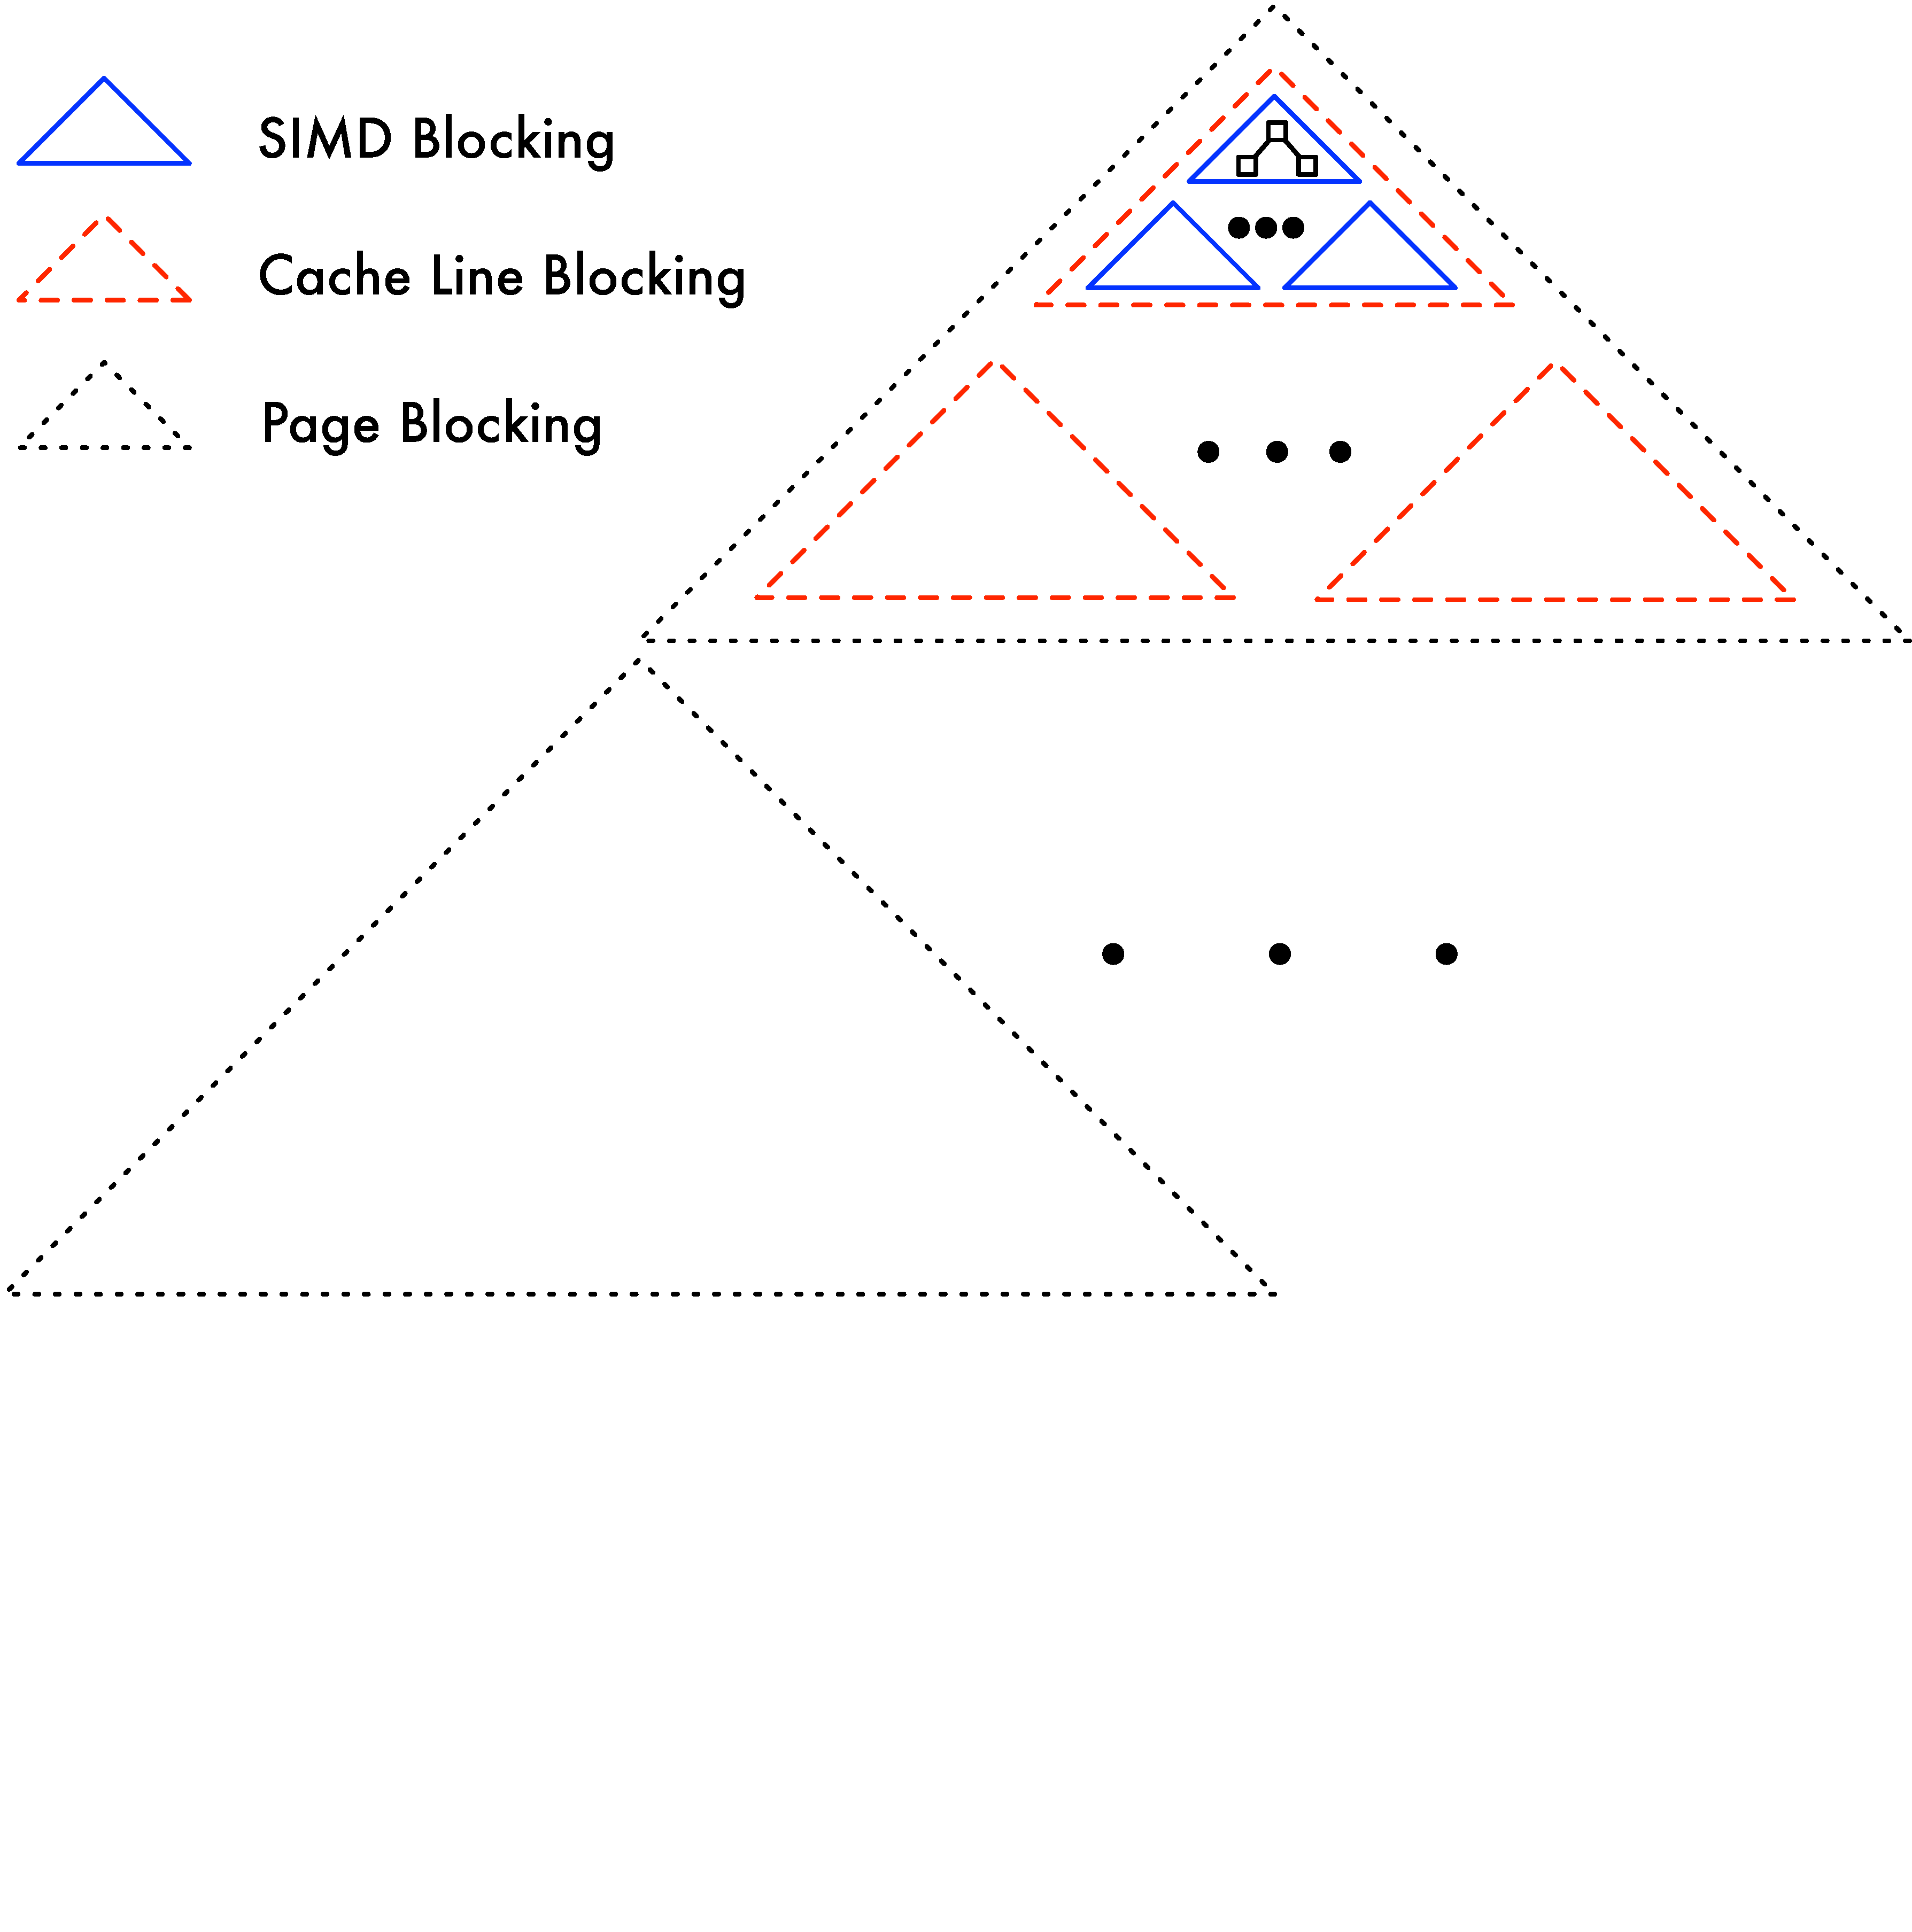
\includegraphics[width=.45\textwidth]{FAST}\vspace{-60pt}
	\caption{Index tree blocked in three-level hierarchy: first-level page blocking, second-level cache line blocking, third-level SIMD blocking of FAST. Adapted from Kim et al. \cite{kim2010fast}.}
	\label{fig}  
	\end{center}
\end{wrapfigure}Kim et al. adapted a binary tree to optimize for architecture features like page size, cache line size, and SIMD bandwidth called Fast Architecture Sensitive Tree \cite{kim2010fast}. In contrast to Seg-Tree, FAST is also adapted to disk-based database systems. Kim et al. show the performance increase because of decreasing cache misses and better cache line usage. In order to optimize for architectural features, tree nodes are rearranged for hierarchical blocking. In Figure 3, we show an index tree blocked in three-level hierarchy introduced by Kim et al. 



% How hierarchical blocking is achieved
According to Figure 3, we define $d_K=2$ as the depth of a SIMD block, $d_L=5$ as the depth of a page block, $N_K=2^{d_K} -1$ as the number of keys that fit into a SIMD register, and $N_L = 2^{d_L} - 1$ as the number of keys that fit into a cache line. To rearrange the nodes, Kim et al. sorted the nodes, as shown in Figure 3 (a). Afterwards, they combine the first $N_K$ keys and lay them out in breadth-first fashion (the first key as root, the next $N_K - 1$ keys as children on depth 2). These first $N_K$ keys represent a SIMD block. They continue to lay out the next keys the same fashion, building the SIMD blocks with root keys 3, 6, 9, and 12, as shown in Figure 3 (b). This process continues for all sub-trees that are completely in the first $d_L$ levels from the root. If a sub-tree does not completely fit in the first $d_L$ levels, the keys are laid out according to the appropriate number of levels $(d_L \% d_K)$ as shown in depth 4 in Figure 3 (b). The first $N_L$ keys represent a cache line block. We define $d_P=31$ as the depth of a page block and $N_P=2^{d_P} -1$ as the number of keys that fit into a page. The procedure of hierarchical blocking continues analogue until the $N_P$ keys are laid out, representing a page block. After building one page block, the next page block is build up the same way. In Figure 3 (c) we show the different blocks in a hierarchical blocked index tree.

% Building the tree and search algorithms
Kim et al. present implementations for building and traversing the tree adapted for CPU and also for GPU. Building up the tree, SIMD is used to computing the index for $N_K$ keys within the SIMD level block in parallel, achieving around 2X SIMD scaling as compared to the scalar code. With a Core i7 processor, the runtime of building a FAST tree with $64M$ tuples is less than $0.1$ seconds. Traversing the tree, they compare one search key to multiple keys of the index structure. To use the complete bandwidth of cache and main memory within the search, blocks are loaded completely into associated memories from large blocks to small blocks. For a page block, at first the page is loaded into main memory. Then cache line blocks are loaded one after another in the cache and for each cache line block, the included SIMD blocks are loaded into the SIMD register. All keys of this SIMD block are compared with one SIMD instruction. After looking up the resulting bitmask, the corresponding SIMD block is loaded (including the load of the surrounding larger blocks) until the key is found or the last level of the index structure is reached.

% Performance
Kim et al. consider the search performance as queries per second. The CPU search performance on the Core i7 with 64M 32-bit (key, rowID) pairs is 5X faster than the best reported number \cite{schlegel2009k}, resulting in a throughput of 50M search queries per second. Considering larger index structures, the GPU performance increase exceeds the CPU performance increase, because TLB and cache misses grow up and the CPU search becomes memory bandwidth bound.

% Mention Compression?
\subsection{VAST}\label{SCM}
% What is from FAST
Yamamuro et al. extended FAST building an index structure called Vector-Advanced and Compressed Structure Tree (VAST) \cite{yamamuro2012vast}. They adapt the blocking and aligning structure of FAST and add compression of nodes along with improved SIMD usage. In Figure 4, we show the structure of the VAST-Tree including layers and different blocking elements. The top layer $P_{32}$ uses the techniques of FAST with the same SIMD, cache line and page blocking with 32 bit keys.

% Block compression
In order to decrease the size of the index structure to better fit into main memory, the middle and bottom layers use compressed nodes. In the layer $P_{16}$, the 32 bit keys of each node are compressed to 16 bit keys using lossy compression. Analogue, in $P_8$ the keys are compressed to 8 bit with lossy compression. In the leaf nodes, Yamamuro et al. decrease the node size with the lossless compression algorithm \emph{P4Delta}, which results in a good balance between compression ratio and decompression speed. If an error occurs due to information loss, they present an algorithm for error correction. They use prefix and suffix truncation to compress keys and calculate an offset $\Delta w$ of the incorrect key to the correct key during tree traversal. If $\Delta w\neq0$, VAST-Tree scans the leaf nodes sequentially until $\Delta w$ becomes $0$.

% SIMD usage
Along with the other considered index structures, Yamamuro et al. compare multiple keys to one search key with SIMD in the tree traversal. Due to the key compression of nodes, the VAST-Tree compares more keys in parallel than FAST. Additionally, they reduce branch misses with an adapted SIMD usage. They use addition and multiplication operations on the results of a SIMD key comparison, instead of conditional branches (if-then paths), to find the next node in tree traversal.

% Performance
Due to lossy and lossless compression of the majority of nodes, Yamamuro et al. reach a 95\% less space consumption of the VAST-Tree compared to a binary tree or FAST. When considering an index with $2^{32}$ keys, they reach up to $6.0$ and $1.24$ times performance increase compared to a binary tree and FAST. Although errors occur due to lossy compression, the error correction does not take a major influence on the traversal speed.

%\begin{figure}
%	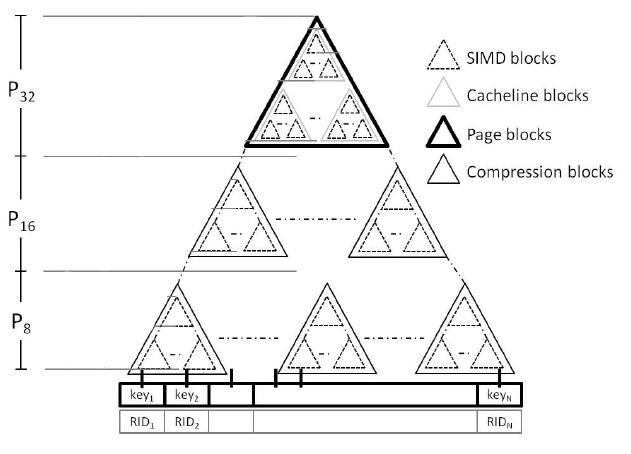
\includegraphics[width=0.5\textwidth]{figure_5.png}
%	\caption{An overview of VAST-Tree. The top layer ($P_{32}$) of VAST-Tree uses FAST techniques, and VAST-Tree compresses the middle and the bottom layers ($P_{16}$ and $P_8$) of the trees. Moreover, keys in leaf nodes ($key_1, key_2, ...,	key_N$) are compressed by using lossless compression. Adapted from Yamamuro et al. \cite{yamamuro2012vast}.}
%	\label{fig}
%\end{figure}


\subsection{ART}\label{SCM}
% Basics about radix tree
Leis et al. adapted a radix tree for efficient indexing in main-memory database systems called Adaptive Radix Tree \cite{leis2013adaptive}. Similar to the Seg-Trie, the height of a radix tree depends on the chunk size of the keys stored in each node. ART divides keys into 8-bit chunks. They differentiate between inner nodes and leaf nodes and adapt each of them in a different way.

% Adaption of inner nodes
Instead of using a constant node size for each inner node, they present four types of nodes with different numbers of keys and children. The types of nodes, sorted ascending by their size, are \emph{Node4}, \emph{Node16}, \emph{Node48}, and \emph{Node256}. When the capacity of a node is exhausted due to insertion, it is replaced by a larger node type. When a node becomes underfull due to key removal, it is replaced by a smaller node type. In Figure 5, we show these node types containing keys that are mapped to subtrees.

% Inner node types
\textbf{Node4}: The smallest node type consists of one array with up to four sorted keys and another array with up to four children. The keys and pointers are stored at corresponding positions.

\textbf{Node16}: This node type consists of arrays of 16 keys and 16 children, storing keys and children analogue to \emph{Node4}.

\textbf{Node48}: To avoid searching keys in many elements, this node type does not store the keys explicitly. Instead, an array with 256 elements is used. This array can be indexed with key bytes directly. It stores indexes into a second array with the size of 48 elements containing the pointers to child nodes.

\textbf{Node256}: The largest node type is simply an array of 256 pointers. Consequently, the next node can be found efficiently using a single lookup of the key byte in that array. 

% Leaf Node implementation
For leaf nodes, Leis et al. use a mix of pointer and value slots in an array. If the value fits within the slot, they store it directly in the slot. Otherwise, a pointer to the value is stored. They tag each element with an additional bit indicating if a pointer or a value is stored.

% SIMD usage
According to FAST and Seg-Tree, Leis et al. use SIMD within the tree traversal. They use horizontal vectorization, comparing the search key against multiple keys of a node. In contrast to Zeuch et al., using horizontal vectorization for each inner node, Leis et al. only compare the keys of nodes with type \emph{Node16} in parallel. Therefor, they replicate the search key 16 times and compare these against all keys of nodes of type \emph{Node16}.

% Space consumption
In contrast to FAST and Seg-Tree, the goal of ART is also to reduce space consumption. Leis et al. use lazy expansion and path compression. The first technique, lazy expansion, is to create inner nodes only if they are required to distinguish at least two leaf nodes. The second technique, path compression, removes all inner nodes that have only one child.

% Performance increase
Since SIMD is only used in the tree search, we do not consider the performance increases of ART in insert and update operations. Leis et al. show, that looking up random keys using ART is faster than Seg-Tree and FAST, because ART has less cache misses and less CPU cycles per comparison. They consider the performance increases for dense and sparse keys, whereas ART works better with dense keys. Also they show that a span of 8 results in better performance than a smaller span. 

\begin{figure}
	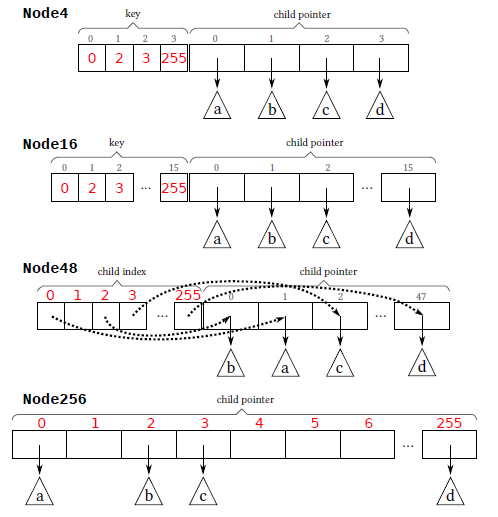
\includegraphics[width=0.5\textwidth]{figure_4.png}
	\caption{Inner nodes of ART. The partial keys 0, 2, 3, and 255 are mapped to the subtrees a, b, c, and d. Adapted from Leis et al. \cite{leis2013adaptive}}
	\label{fig}
\end{figure}


\section{Evaluation}
% What we want to do:
In this section, we define criteria to compare the adaptions made in Seg-Tree, FAST, ART, and VAST to increase performance and show differences. We primarily focus on the usage of SIMD within the adapted index structures. %All considered adaptions have the following points in common:
In Table 2, we show the performance criteria and their impact on performance increase and show which index structure implements which of the criteria. In the following, we consider each criterium in detail before summarizing the comparison. For each criteria, we show how the index structure implements it. If the index structure does not implement the criteria, we consider if it is possible to implement it. Furthermore, we constitute why the adaptions cannot compared directly in view of performance.

\begin{table*}[htbp]
\footnotesize
	\caption{Comparison of the considered index structures based on extracted criteria and the impact on performance increase}
	\begin{center}
		\begin{tabular}{|c|c|c|c|c|c|}
			\hline
			\textbf{Criterium}&\textbf{Seg-Tree/Trie}&\textbf{FAST}&\textbf{ART}&\textbf{VAST}&\textbf{Impact}\\
			\hline
			Horizontal vectorization & x & x & x & x & high\\
			Minimized key size & o & - & x & x & high\\
			Adapted node sizes and types & - & x & - & x & low\\
			Decreased branch misses & - & x & - & x & medium\\
			Full use of cache line using blocking and alignment & - & x & - & x & medium\\
			Usage of Compression & o & - & x & x & medium\\
			Adapt search algorithm for linearised nodes & x & - & - & - & low\\
			\hline
			\multicolumn{6}{|c|}{Legend: x = implements the issue; o = partially implements the issue; - = does not implement the issue}\\
			\hline
		\end{tabular}
		\label{tasuaib2011architecture}
	\end{center}
\end{table*}

\subsection{Horizontal Vectorization}
% Reason for the performance issue
Segmenting the index structure is important to reach a better performance increase with SIMD instructions. Since the data for a SIMD operation has to be stored sequentially in main memory, a good segmenting and blocking strategy is necessary. In Section 2, we present the vertical vectorization as alternative to horizontal vectorization. Due to the necessity of sequential data storage in main memory, comparing a different search key per vector lane is not applicable for SIMD instructions in tree traversal. All considered adaptions use horizontal vectorization in search operation for a single search key in the index structure.

% Decreasing Branch misses with addition/multiplication operations
The search performance also depends on the evaluation of a comparison with SIMD operations. Kim et al. and Zeuch et al. use conditional branches (if-then paths) within their search algorithms, which leads to more branch misses compared to the approach of Yamamuro et al. They perform addition and multiplication operations on the bitmask to avoid branch misses for better search performance. This approach can also be applied on Seg-Tree/Trie and ART to reduce branch misses.

\subsection{Minimized key size}
%- Zeuch et al. small key sizes for Seg-Tree, Art small chunks and VAST uses compression.
% Reason for the performance issue
Minimizing the key size as much as possible speeds up the search performance, because more keys can be compared with a single SIMD instruction. Additionally, the smaller the keys are, the more keys fit into a cache line. Since tries or radix trees, depending on their span, have small chunks of the search key in each node, more keys are compared in parallel.

% Seg-Tree/Trie and ART
Zeuch et al. minimize the key size for the Seg-Trie using a small chunk size. This leads to a bigger tree height, but the performance increase of comparing more keys in parallel leads to better search performance. For the Seg-Tree, they do not use adaptions to minimize the key size, therefore the performance increase with SIMD depends on the size of the used data type. Analogue to the Seg-Trie, Leis et al. use a small key size for ART to increase the performance speed up.

% FAST and VAST
Kim et al. do not minimize the key size for FAST, therefore the performance increase with SIMD also depends on the size of the used data type. Yamamuro et al. use compression to minimize the key size of VAST, respectively to the layer. Since VAST is an extended Version of FAST, there is no need to check if this adaption is also applicable for FAST. 

%If keys are stored completely in one node, like in Seg-Tree and FAST, Yamamuro et al. show that compression of keys results in better search performance [5]. Zeuch et al. show

\subsection{Adapted node sizes and types}
% Reason for the performance issue
Index structures for disk-based database systems often adapt their node size to the page size of disk. In modern database systems, this adaption becomes obsolete. Consequently, the considered index structures adapt their node to other parameters. 

% Seg-Tree/Trie
Zeuch et al. adapted the $B^+$-Tree by having a k-ary search tree as each inner node. To perform k-ary search on the keys of a node, each node has the size of multiple of the SIMD-bandwidth $k$.

% FAST and VAST
Kim et al. segment FAST into SIMD, cache, and page blocks. Each block contains multiple nodes, respectively to the block size. Since FAST is based on binary tree, every node contains still a single element and is not adapted in type or size. VAST uses the same hierarchical blocking and also does not adapt single nodes.

% ART
Leis et al. present different node types for inner nodes of ART. The node types differ in the number of keys and child nodes. 

\subsection{Decreased branch misses}
% Reason for the performance issue
Evaluating the result of a comparison with SIMD using conditional branches can lead to branch misses, if the CPU prefetches the wrong branch. Consequently, decreasing branch misses improves search performance because less CPU cycles are needed. Yamamuro et al. use addition and multiplication operations in VAST to find the next node in their evaluation of the comparison result. This avoids conditional branching and therefore decreases branch misses.

% Seg-Tree and Seg-Trie
Zeuch et al. use conditional branches in their search algorithms for the Seg-Tree and Seg-Trie, which can be replaced by the approach of VAST to decrease branch misses. Analogue, ART can be adapted using this approach to speed up the search performance.
\subsection{Full use of cache line using blocking and alignment}
% Reason for the performance issue
Due to in-memory database systems, the IO-bottleneck moves from disk to RAM further to RAM to cache. Consequently, an efficient cache line usage is important to speed up the performance of index structures. An efficient cache line usage is reached by blocking parts of index structures to cache line size.

% Seg-Tree/Trie
Zeuch et al. linearise keys to a multiple of the SIMD bandwidth with the Seg-Tree but not adapt the node size to the cache line size. Accordingly, an adaption of the inner nodes of Seg-Tree to the cache line size could lead to better cache line usage and consequently to better search performance. 

% Fast and VAST
Kim et al. segmented FAST into SIMD, cache, and page blocks. They highly optimize FAST for efficient cache line usage by blocking the index structure into blocks with the size of a cache line.

% ART
Leis et al. also do not make adaptions of ART in view of blocking to the cache line size. Thus, a performance increase can be reached by adapting ART to cache line size.
\subsection{Usage of compression}
% Usage and type of compression
Along with the fast growing amount of data stored in modern database systems, the size of index structures grows fast. Compression of nodes decreases the size of index structures. Key compression leads to better search performance with SIMD, because more keys are compared in parallel.

%Seg-Tree and FAST
Zeuch et al. do not use any node or key compression for Seg-Tree. Kim et al. also do not compress nodes or keys in FAST. Consequently, considering compression for Seg-Tree and FAST provides space for additional performance increase.

% VAST
Yamamuro et al. use lossy block compression to decrease the key size of blocks. Consequently, they compare more keys with one SIMD instruction, whereas performance decrease of the occurring errors is smaller than the performance increase of the compression. Instead of compressing blocks, Seg-Trie and ART use path compression to decrease the tree height. Consequently, less nodes are passed to reach the matching leaf node, if it exists.
% ART
Leis et al. use path compression within ART. Path compression removes all inner nodes that have only one child to decrease the tree height and therefore increase search performance. Key compression is a possible adaption for ART to improve the search performance.

\subsection{Adapt search algorithm for linearised nodes}
% Reason for the performance issue
Searching children in nodes with many keys can be speeded up with adapted search algorithms compared to linear search.

% Seg-Tree and Seg-Trie
Zeuch et al. introduce k-ary search for the Seg-Tree and Seg-Trie, which performs in $O(log_n)$ compared to $O(n)$ of linear search, where $k$ is the SIMD bandwidth. Consequently, less keys are compared in one node, whereas a linearised storage of the keys in the node is required. 

% FAST, ART 
For FAST and VAST, the k-ary search is not applicable because they are adapted from binary trees and have only one key in each node. Leis et al. use linear search in their adapted nodes of ART to find children. For the node type \emph{Node256} k-ary search can speed up finding the correct child node. Therefore ART provides space to use k-ary search for this node type.

\subsection{Summary}
%- Commons and differences\\
%- Conclusion: Maybe weighting the points

After considering each performance criteria in detail, we summarize the comparison and weight the mentioned criteria according to their performance increase. 

% Horizontal vectorization
%Since the data for a SIMD operation has to be stored sequentially in main memory, all adapted index structures use horizontal vectorization to compare multiple keys in parallel, but use different approaches to evaluate the result of the SIMD comparison. 
As mentioned before, comparing a different search key per vector lane is not applicable for SIMD instructions in tree traversal. Therefore, all considered adaptions use horizontal vectorization, but evaluate the result of the SIMD comparison in different ways. Since horizontal vectorization with SIMD, depending on the key size, leads to direct performance increase up to a multiple, we assign the highest weight to it. 

% Minimize key size
Due to the mentioned performance increase of horizontal vectorization, minimizing key size also leads to better search performance. We assign the second highest weight to minimizing the key size, since more keys are compared in parallel. Because of the compression of keys, VAST reaches the highest performance increase by minimizing key size compared to the other index structures. 

% Cache line usage and branch misses
Compared to horizontal vectorization and minimizing key size, an efficient cache line usage and avoiding branch misses lead to lesser performance increase. Although, both criteria decrease the number of CPU cycles, the performance increase does not reach a multiple. Therefore, we assign the third highest weight to efficient cache line usage and to avoiding branch misses.

% Compression
Afterwards, we assign the fourth highest weight to the usage of compression. With key compression, the performance increase of horizontal vectorization rises. Path compression decreases the height of index structures and consequently less nodes are passed during traversal. 

% Adapted node types and adapted search algorithm
We assign the lowest weight to the adaption of nodes and to the usage of an adapted search algorithm. The adaption of nodes does not lead directly to performance increase, but is the basis for horizontal vectorization and efficient cache line usage. The usage of an adapted search algorithm, for example k-ary search, needs lesser comparisons. Nevertheless, it is not applicable for all of the considered index structures and it requires large node sizes to increase the performance.  

% Performance comparison
Although our qualitative comparison yields various structural differences of the index structures, we cannot infer unbiased performance differences from the literature. The performance increases highly depend on the underlying hardware, the data types chosen for the keys, and the amount of keys inserted in the index structure. Therefore, comparing all structures directly does not lead to reasonable results. Although, Yamamuro et al. and Leis et al. compare VAST \cite{yamamuro2012vast} and ART \cite{leis2013adaptive} to FAST, they only consider specific key sizes and data types. 

% GPU calculation, cache line usage becomes different impact, completely different technology%
%At last, we consider the usage of SIMD with the GPU. Zeuch et al. and Kim et al. present algorithms to use GPU calculation for the Seg-Tree/Trie [3]. They compare one search key against multiple other keys with SIMD registers in the GPU, analogue to CPU usage. Since passing data to GPU registers is completely different compared to CPU registers and the other index structures only use the CPU, we do not go further into details of CPU calculation with SIMD. \textbf{TODO: References for SIMD with GPU?}
% In Common:
%\begin{itemize}
%	\item Keep the key size as small as possible, to compare more keys in parallel
%	\item Adapt node sizes and types for a better usage of SIMD registers and cache lines
%	\item Use SIMD instructions to compare the search key with multiple keys of the index
%\end{itemize}

% Small keys, to compare more in parallel
%Before looking at the differences, we go into detail for each entry of the list. At first,
% Segmenting the tree

% SIMD usage
%At last, we consider the usage of SIMD of the index structures. 

%Differences
%Furthermore, we present the following differences in the adaptions of the index structures:
%\begin{itemize}%
%	\item Usage and type of compression
%	\item FAST and Seg-Tree are read-only, ART and FAST implement update and delete operations
%	\item Usage of GPU instead of CPU calculation
%\end{itemize}

% Read-Only vs Read-Write
%Since all considered index structures use SIMD only for tree traversal, Zeuch et al. and Changkyu et al. present the Seg-Tree/Trie and FAST as read-only, which means they do not show adapted update or delete operations. For statistical usage or data warehouses, update and delete operations are not required and read-only index structures serve the purpose. To fulfill the requirements of general index structures, Leis et al. and Yamamuro et al. also present update and delete operations for ART and VAST. Both using the performance increase of tree traversal with SIMD for these operations, because the matching node for the search key has to be found in the tree.

\section{Related Work}
% B+ Tree adaptions, compression
In main-memory database systems, a $B^+$-Tree does not fulfill the requirements of efficient cache line usage. Therefore, it is important to adapt $B^+$-Trees to efficient cache line usage. Rao et al. show improved cache line usage for $B^+$-Trees \cite{rao1999cache}.  Compression is used to decrease the index size to fill more keys into the cache line. Zukowski et al. show the performance increase of better cache line usage with compression \cite{zukowski2006super}. This adaption gives an alternative for us compared to the compression used in VAST.

% Other adapted tree strucutures
Graefe et al. present and summarize several techniques for improving cache performance for B-Trees \cite{graefe2001b}. Furthermore,
Bender et al. show a cache oblivious B-Tree \cite{bender2000cache} and a cache oblivious B-Tree for string data types \cite{bender2006cache}. Other adapted index structures are shown by Rao et al., the Cache-Sensitive Search Trees (CSS-Tree) \cite{rao1999cache}, and the Cache Sensitive $B^+$-Tree (CSB+-Trees) \cite{rao2000making}. They construct the tree such that the keys are placed with the best cache optimization as possible in terms of spatial or temporal locality. Since we consider efficient cache line usage as an important criteria for modern index structures, these adaptions gave useful ideas to measure performance increase due to efficient cache line usage. 

% SIMD usage, vectorization
During the traversal of an index structure in modern database systems, a huge number of keys are compared. Consequently, using SIMD instructions leads to better search performance. Polychroniou et al. consider different techniques to process multiple data items with one SIMD instruction \cite{polychroniou2015rethinking}. They differentiate between horizontal and vertical vector processing and present benefits of each approach. We use this differentiation of vector processing for our comparison of SIMD usage.  

% k-ary search
To compare as less keys as possible within one node to find the matching children, Zeuch et al. show the performance increase using k-ary search with SIMD instructions \cite{zeuch2014adapting}. Schlegel et al. present the general benefits of k-ary search on modern processors \cite{schlegel2009k}. Since k-ary search leads to a considerable factor of lesser key comparisons for large nodes, we choose the usage of an adapted search algorithm as one of our performance criteria.

% Comparison of adapted index structures
Comparing adapted index structures for modern database systems leads to find important points to increase the performance of index structures. Yamamuro et al. and Leis et al. compare VAST \cite{yamamuro2012vast} and ART \cite{leis2013adaptive} to FAST and show a performance increase. We consider this comparison to weight our performance criteria.

\section{Conclusion and Future Work}

% What changes
%Index structures which were designed for disk-based memory database systems does not fulfill the requirements of modern database systems. Due to in-memory database systems, the IO-bottleneck moves from disk to RAM further to RAM to cache. Furthermore, not only the number of CPU cycles restricts the performance, also cache and branch misses have an important impact of performance. Modern CPUs provide multiple SIMD registers and instructions to process multiple data items in parallel. Using SIMD speeds up the performance, depending on the implementation of the operations with SIMD.

% Say what you say before you say it
In this work, we compare the adapted index structures Seg-Tree/Trie, FAST, VAST, and ART and evaluate the usage of SIMD within these. We extract important criteria of these adaptions and weight them according to their impact on the performance.

% Important criteria
Due to direct performance increase of horizontal vectorization with SIMD up to a multiple, this is the highest weighted criteria. Minimizing the key size leads to the comparison of more keys in parallel and is therefore assigned with the second highest weight. Afterwards, we assign the efficient usage of the cache line and the decrease of branch misses the third highest weight. The other considered criteria, in descending order in view of performance increase, are the usage of compression, the adaption of node types and size, and the usage of an adapted search algorithm to find keys within nodes. 

% Space for additional improvements of some index structures
Since not all considered index structures implement all criteria, we plan to combine different approaches. We presented that key compression leads to considerable performance increase. Therefore, we plan to examine the usage of key compression for Seg-Tree and ART. Furthermore, we plan to apply the evaluation of SIMD comparison results with addition and multiplication operations used in VAST to Seg-Tree and ART. 

At last, we plan to examine the usage of k-ary search in ART for the node type \emph{Node256}, since the other node types contain too less keys to get a considerable performance increase. 
%\begin{itemize}
%	\item Horizontal vectorization
%	\item Minimized key size
%	\item Adapted node sizes and types
%	\item Decreased branch misses
%	\item Full use of cache line using blocking and alignment
%	\item Compression
%	\item Adapt search algorithm for linearised nodes
%\end{itemize}

%- Weighting of important points, descending\\
%$\rightarrow$ Keep keys as small as possible because comparing keys in parallel leads to direct performance speed up\\
%$\rightarrow$ Save space with compression\\
%$\rightarrow$ Align and block the index structures for better cache line usage\\
%$\rightarrow$ Decrease branch misses like VAST do\\

%\section{Future work}
%\begin{itemize}
%	\item Using k-ary search in FAST/VAST
%	\item Looking in detail to the decrease of branch misses using addition/multiplication operations and SIMD
%	\item Another use of SIMD in index structures than search, other DB operations
%	\item Look at other SIMD techniques and parameters to increase performance
%\end{itemize}

%BDAS conference
%this is the place where you include the bibliography in a separate file
%add both lines - ref_1284 is a name of your bib file
\bibliographystyle{splncs}
\bibliography{SIMD_Acceleration_for_Index_Structures} 

\end{document}
